%!TEX root = ../docu.tex
\section{Konzept}
\subsection{Grundkonzept}

Im folgenden wird die Kozeptionierung der Anwendung beschrieben, welche im späteren implementiert wird. Hierbei handelt es sich um eine Applikation hauptsächlich für das abspielen von Hörbüchern im Audioformat MP3. Die Applikation soll so einfach wie möglich gestaltet und zweckgerichtet sein.

Die Applikation soll dem Benutzer ermöglichen Hörbücher abzuspielen, welche er vorher auf sein mobiles Endgerät abgelegt hat. Hierfür muss die Applikation einen Einstellungsmöglichkeit beinhalten.

Über diese Einstellungen muss es dem Benutzer möglich sein den Speicherort frei wählen zu können. Über diese Einstellungsparameter ist es der Anwendung nun möglich alle Audiodateien aufzulisten und abspielen zu können.

Die Auflistung filtert alle nicht abspielbaren Daten und ermöglicht des Weiteren in Unterordnen zu navigieren. Ein Element der Liste stellt dabei entweder eine Audiodatei oder ein Unterordner dar. 

\begin{figure}
\begin{center}
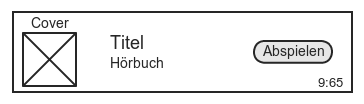
\includegraphics[scale=0.8]{images/listitem}
\caption{Mockup für ein Listenelement}
\label{mocklistel}
\end{center}
\end{figure}

Die Abbildung \ref{mocklistel} beschreibt ein solches Element. Ein Element enthält das Cover des Hörbuches sowie der Title und die genau Abspielzeit. Über ein weiteres Element soll es möglich sein eine Aktion auszuführen, welche das Abspielen der jeweiligen Audiodatei ermöglicht.

Aus dieser Auflistung heraus soll es möglich sein Audiodateien abspielen zu können. Deshalb muss eine Schnittstelle zur Übertragung der Informationen zur Player Komponente erfolgen.

Diese Komponente ist für das abspielen zuständig. Sie empfängt die Anweisung zum Abspielen der Audiodatei und spielt dieses Datei letztendlich ab.

\begin{figure}
\begin{center}
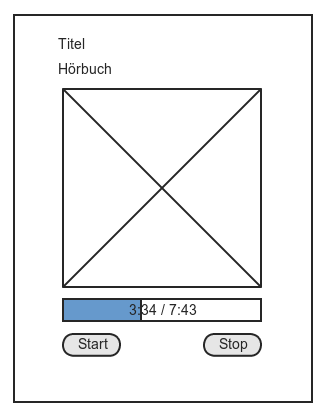
\includegraphics[scale=0.6]{images/playerkomp}
\caption{Schematische Darstellung der Abspiel-Komponente}
\label{playerkomp}
\end{center}
\end{figure}

Die Player Komponente in Abbildung \ref{playerkomp} dargestellt, soll es ermöglichen das Abspielen zu steuern. Dies beinhaltet das Stoppen, Pausieren und andere Funktionen. Des Weiteren soll Erkennbarkeit sein welche Audiodatei abgespielt wird. Eine Vorschrittanzeige lässt erkennen, wie viel von der Audiodatei bisher abgespielt wird sowie die Gesamtlänge der Audiodatei.

\begin{figure}
\begin{center}
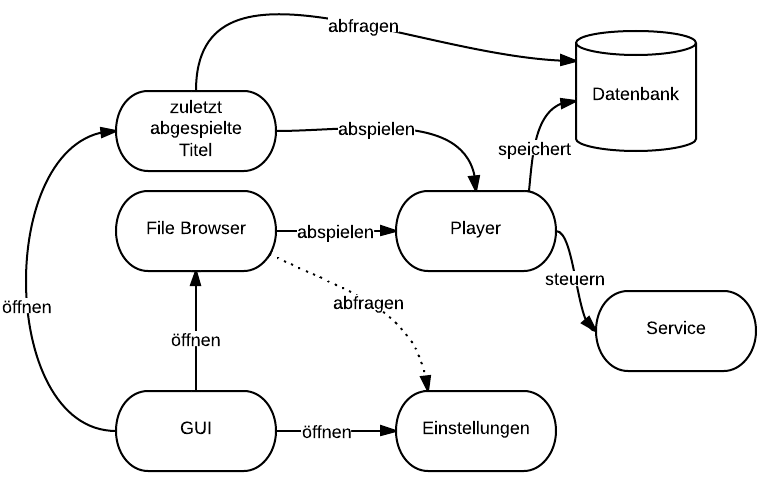
\includegraphics[scale=0.6]{images/konzept}
\caption{Schematische Darstellung der Anwendung}
\label{konzept}
\end{center}
\end{figure}

Wird die Anwendung geschlossen soll die Wiedergebe abbrechen. Sie soll in der Lage sein Abbrüche der Wiedergabe zu erkennen und diese Punkte zu Speicher. Der Benutzer soll aus diesen Informationen eine Möglichkeit haben, an diesen Punkten die Wiedergabe vorzusetzen.

Die Eingabe erfolgt durch ein übliches Touchscreen Display und sollte dahingehen optimiert sein. Hierzu gehört klare und einfache Programmstrukturen sowie ausreichend große fälschen für Bedienelemente und Steuerung von Programmfunktionen.

Die gesamte Programmstruktur muss so aufgebaut sein, um eine Weiterentwicklung und Implementierung neuer Funktionen zu ermöglichen.
